\de{
Sei $ABC$ ein Dreieck mit $\angle CAB = 2\cdot\angle ABC$. Nehme an, dass ein Punkt $D$ im Inneren des Dreiecks $ABC$ existiert, sodass $AD = BD$ und $CD = AC$. Zeige, dass  $\angle ACB = 3\cdot\angle DCB$.

\textbf{Lösung:} (David)
\begin{center}
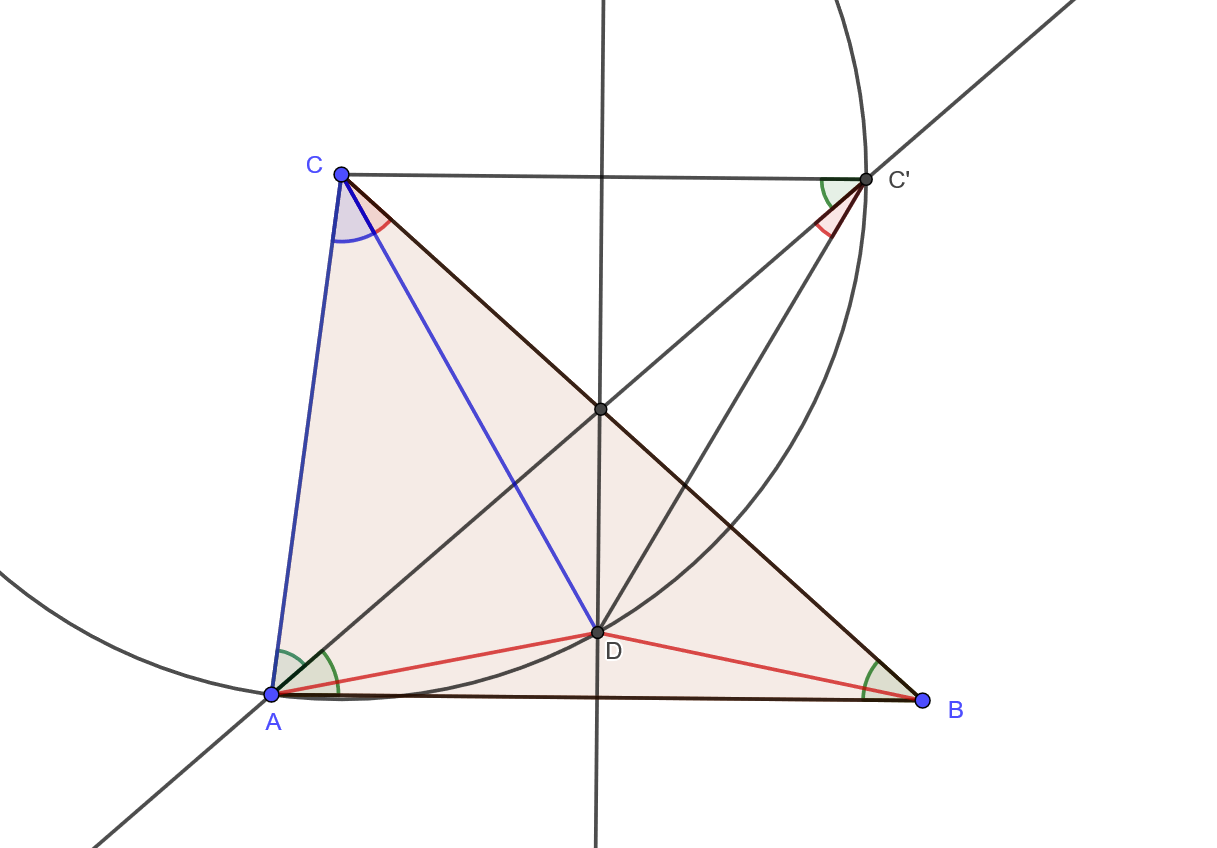
\includegraphics[width=0.8\textwidth]{f7_picture.png}
\end{center}
\vspace{0.8cm}
Wir wollen zunächst etwas mehr über die geometrische Situation dieser Aufgabe herausfinden:
Damit $AD=BD$ gelten kann, muss $D$ auf der Mittelsenkrechten von $AB$ liegen. \\ Aus $CD=AC$ folgt, dass $D$ auf einem Kreis mit Mittelpunkt $C$ und Radius $AC$ liegt. Damit ist $D$ der Schnittpunkt dieser beiden Objekte.
Zudem suggeriert uns die Bedingung $\angle CAB = 2 \angle ABC$, dass die Winkelhalbierende von $\angle CAB$ eine wichtige Rolle spielen könnte. Sei $C'$ der Schnittpunkt dieser Winkelhalbierenden mit dem Kreis mit Radius $AC$ um $C$. Wegen $CA=CC'$ gilt
\[ 
\angle AC'C = \angle CAC' = \frac{1}{2} \angle CAB = \angle ABC. \]
Also sehen wir mit der Umkehrung des Peripheriewinkelsatzes, dass $ABC'C$ ein Sehnenviereck ist. Des weiteren wissen wir sogar, dass $\angle BAC' = \angle C'AC = \angle CC'A$ gilt. Folglich ist $CC'$ parallel zu $AB$ und damit $ABC'C$ ein gleichschenkliges Trapez.
\\
Mit dieser Beobachtung können wir nun wieder die Mittelsenkrechte $m$ von $AB$ ins Spiel bringen: Sie ist nämlich die Symmetrieachse des Trapezes $ABC'C$. Da $D$ auf der Symmetrieachse liegt, gilt $\angle BCD = \angle DC'A$. Das ist nützlich, weil $C'$ auf unserem Kreis liegt. Wir müssen jetzt nur noch den Zentriwinkelsatz anwenden und sehen $\angle ACD = 2\cdot \angle AC'D = 2 \cdot \angle DCB$, also 
\[
\angle ACB = \angle ACD + \angle DCB = 2 \cdot \angle DCB + \angle DCB = 3 \cdot \angle DCB.
\]

\textbf{Note:}(Arnaud) It's a beautiful geometry problem. Like David emphasized in his proof, you have to think big. Clearly, the initial configuartion is quite restricted (in the sense that the picture seems not complete). David suggested to complete the trapezoid with the point $C'$. You could also think even bigger and complete the isoceles triangle with base $AB$ and $C$ lying on one of the side. This basically kills the problem.

\textbf{Marking Scheme:}
\begin{itemize}
    \item +1P: Dessiner $C'$ et le nommer
    \item +2P: Définir $C'$ et montrer un fait non-trivial sur $C'$. Ce fait peut par exemple être:
    \begin{itemize}
        \item Montrer que $C'$ est sur la bissectrice en $A$.
        \item Montrer que $C'$ est sur la parallèle à $AB$ par $C$.
        \item Montrer que $C'$ est sur le cercle de rayon $CA$ et de centre $C$.
        \item Montrer que $C'$ est sur le cercle circonscrit d'$ABC$.
        \item Montrer que $C'$ est sur la médiatrice de $BC$.
        \item Montrer que $C'$ est le symétrique de $C$ par rapport à la médiatrice d'$AB$.
        \item Montrer que $CDC'$ forme un triangle équilatéral
        \item Montrer que $C'$ est le centre du cercle circonscrit de $CDB$
    \end{itemize}
    On notera que cette liste est non-exhaustive, et que la non-trivialité de chacune de ces propositions dépendra de la définition que le participant aura faite de $C'$.
    \item +2P: Montrer que $C'$ est sur le cercle de centre $C$ par $A$ et $D$ ainsi que le symétrique de $C$ par rapport à la médiatrice de $AB$.
    \item +2P: Conclure
\end{itemize}
}